\documentclass[
paper=128mm:96mm,
fontsize=12pt,
pagesize,
parskip=half-,
]{scrartcl}

\usepackage[nochapters]{classicthesis}

\renewcommand{\sffamily}{\rmfamily}

\usepackage[top=.25in, left=.5in, right=.5in, bottom=.5in]{geometry}
\usepackage{minted}
\newcommand{\slide}[1]{#1 \clearpage}
\newcommand{\sectionslide}[1]{\slide{\hfill \vfill \section{#1} \vspace{5em}}}
\newcommand{\subsectionslide}[2]{\vspace*{1em}\slide{\subsection{#1} #2}}

\title{Be A Computer Scientist: Game Programming}
\author{Bendell, XX}
\date{}

\usepackage{graphicx}
\usepackage{eso-pic}

\renewcommand{\baselinestretch}{1.1} 

\renewcommand\maketitle
{
	\vspace*{3ex}
	\begin{center}
		{\Huge Be a Computer Scientist \vspace*{.3em} \par}
		{\large Game Programming \par}
		\vspace*{2em}
	\end{center}
}


\usepackage{titlesec}
\usepackage{multicol}

\titleformat*{\section}{\Large}
\titleformat*{\subsection}{\large}

\titlespacing*{\section}
{0ex}{0ex}{0ex}
\titlespacing*{\subsection}
{0ex}{0ex}{0ex}

\begin{document}
	
    %\AddToShipoutPictureBG{
\includegraphics[height=\paperheight]{gfx/background.jpg}}
	
	\slide
	{
		\maketitle	
	}
	
	\sectionslide{Programming Video Games}

	\subsectionslide{Big Budget Games}
	{
		\begin{itemize}
			\item Typically use a complicated game engine
			\item Examples include Unreal Engine (Epic Games), Frostbite (EA), Anvil (Ubisoft)
			\item I'll be showing a little about Unreal Engine
			\item Made by many programmers, graphic designers, 3d modelers
		\end{itemize}	
	}
	
	\subsectionslide{Our Game!}
	{	
		\vspace{4em}
		\begin{center}
			\begin{huge}
				SPACE RACER
			\end{huge}
		\end{center}
	}
	
	\subsectionslide{Our Schedule for the Week}
	{
		\begin{enumerate}
			\item Learn basic programming
			\item Explore 3D modeling
			\item Learn about how the different parts of games fit together
			\item Learn basic AI
			\item Hold a competition!
		\end{enumerate}
	}
	
	\sectionslide{Basic Programming}
	
	\subsectionslide{What is programming?}
	{
		\begin{enumerate}
			\item A computer follows instructions one by one
			\item A \textit{program} is an instruction set
			\item A program might take in \textit{input} from a user
			\item A program often returns \textit{output} the user can see
		\end{enumerate}	
	}
	
	\subsectionslide{Machine Code}
	{
		\begin{itemize}
			\item The computer reads \textit{machine code}
			\item Machine code is hard to write and hard to read
			\item Sometimes we use it for performance
			\item For the most part, we run away from it because the "easy" version of it looks like...
		\end{itemize}	
	}
	
	\slide
	{
		\begin{footnotesize}
		\inputminted{nasm}{code-snippets/helloworld.nasm}
		\end{footnotesize}

	}
	
	\subsectionslide{Higher Level Languages}
	{
		\begin{itemize}
			\item A higher level language lets you write code that gets converted to something the machine understands
			\item The language may also check for errors for you
			\begin{itemize}
				\item Errors at \textit{compile time}
				\item Errors at \textit{runtime}
			\end{itemize}
			\item Easier to understand, the one we'll be using looks like...
		\end{itemize}
	}

	\slide
	{
		\vspace*{2em}
		\inputminted{java}{code-snippets/helloworld.java}
	}
	
	\subsectionslide{Java}
	{
		\begin{itemize}
			\item High level programming language
			\item Good choice if working on simple \textit{cross platform} programs
			\item Is \textit{object oriented}
			\item Can work from the \textit{command line}, but we're going to use an \textit{integrated developer environment}
		\end{itemize}
	}
	
	\subsectionslide{Making a scratch project}
	{
		\begin{enumerate}
			\item Open Eclipse (circular icon left side of screen)
			\item Select "New Project..."
			\item Make New Java Project
			\item Then we're going to make a new class
		\end{enumerate}
	}
	
	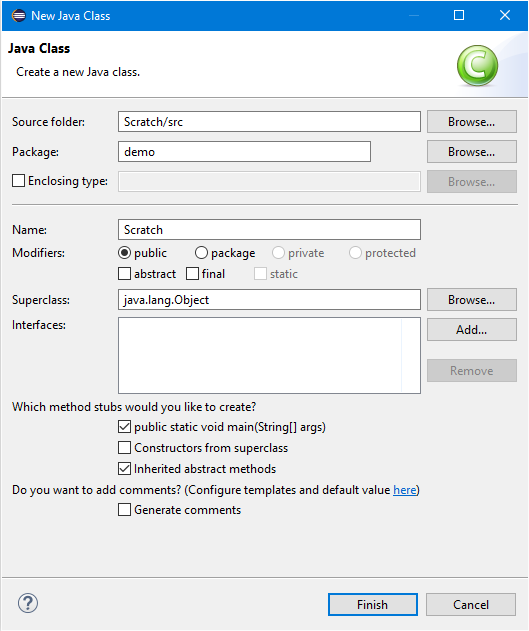
\includegraphics[height=0.8\textheight]{gfx/newjavaclass.png}
	
	\subsectionslide{Variables and Assignment}
	{
		\vspace*{2em}
		\inputminted{java}{code-snippets/variables.java}
	}
	
	\subsectionslide{Types of Variables}
	{
		\vspace*{2em}
		\inputminted{java}{code-snippets/types.java}
	}
	
	\subsectionslide{Programming Together}
	{
		\begin{itemize}
			\item We're going to all program together now
			\item Programming examples will be provided for the lab section
		\end{itemize}

	}
	
\end{document}